\chapter{Feed forward control @@@(Move this?)}

This was never implemented into the controller, which is why it is in the appendix. 

\noindent
An alternative to trying to suppress most disturbances to estimate them through output-measurements, is if they can be measured directly. If the plant is sufficiently well-behaved, then it is possible to make a feed-forward controller that can cancel the effects of the process disturbance. Most feed-forward control is done on SISO\footnote{Single Input, Single Output} systems, like what is seen in  figure \ref{fig:Feed_forward_PID_structure}. In this model, the process dynamics form the controllable input to the output is $P(s)$, the dynamics from the process disturbance to the output is $G(s)$ and the feed-forward controller is $F(s)$, while the feed-back controller is $C(s)$. In a SISO-system, if $P(s)$ has no zeros in the right half-plane the easiest way to make a controller that will cancel the disturbance is by making
\begin{align}
    F(s) = \frac{1}{P(s)}G(s)
\end{align}
But this is usually not possible if any of the zeros are in the right half-plane. The result to this is normally to split $P(s)$ into two $P(s) = P_{mp}(s) P_{nmp}(s)$, where $P_{mp}$ is all the state that make up a phase system\footnote{Minimum phase will mean that all zeroes are in the left half-plane}, while the $P_{nmp}$ only the poles in the right half-plane. It is not possible to get rid of the bad poles, so instead, a set of stable zeros can be used to counteract $P_{nmp} = ( -T_1 s+1)\cdots (-T_n s+1)$. Depending on what $G(s)$ is, some factor $\alpha$ can be chosen as to decide how aggressive the feed-forward controller should be. 

\begin{align}
    F_{\text{not proper}(s) = G(s) \frac{1}{P_{mp}(s)} \frac{1}{(\alpha T_1 s +1) \cdots (\alpha T_n s +1)}
\end{align}

If $P(s)$ has a higher relative degree than $G(s)$, then a set of low-pass filters is also needed to make the feed-forward controller realizable. 

\begin{align}
    F(s) = F_{\text{not proper}(s) \frac{1}{(\tau_{lp,1}s +1)\cdots (\tau_{lp,N} s +1)}
\end{align}
Where $M$ is the difference in relative degrees between the controllers. $\alpha$ should be chosen such that the feed-forward controller is not too careful as to not have any effect at all, but also so that the input does not cause an over-correction in the other direction. The initial value-theorem can give an indicator as to how the plant might react to the sudden change. By replacing all $s$ with $\omega \rightarrow \infty$ and allowing, it is possible to see what the initial value to an impulse-response will be. In the case of this project, $G(s)$ is rather slow, and would be able to correct for a lot the reaction in the opposite direction. As a result, $\alpha =0$ would possibly be a decent choice. 
\begin{figure}
    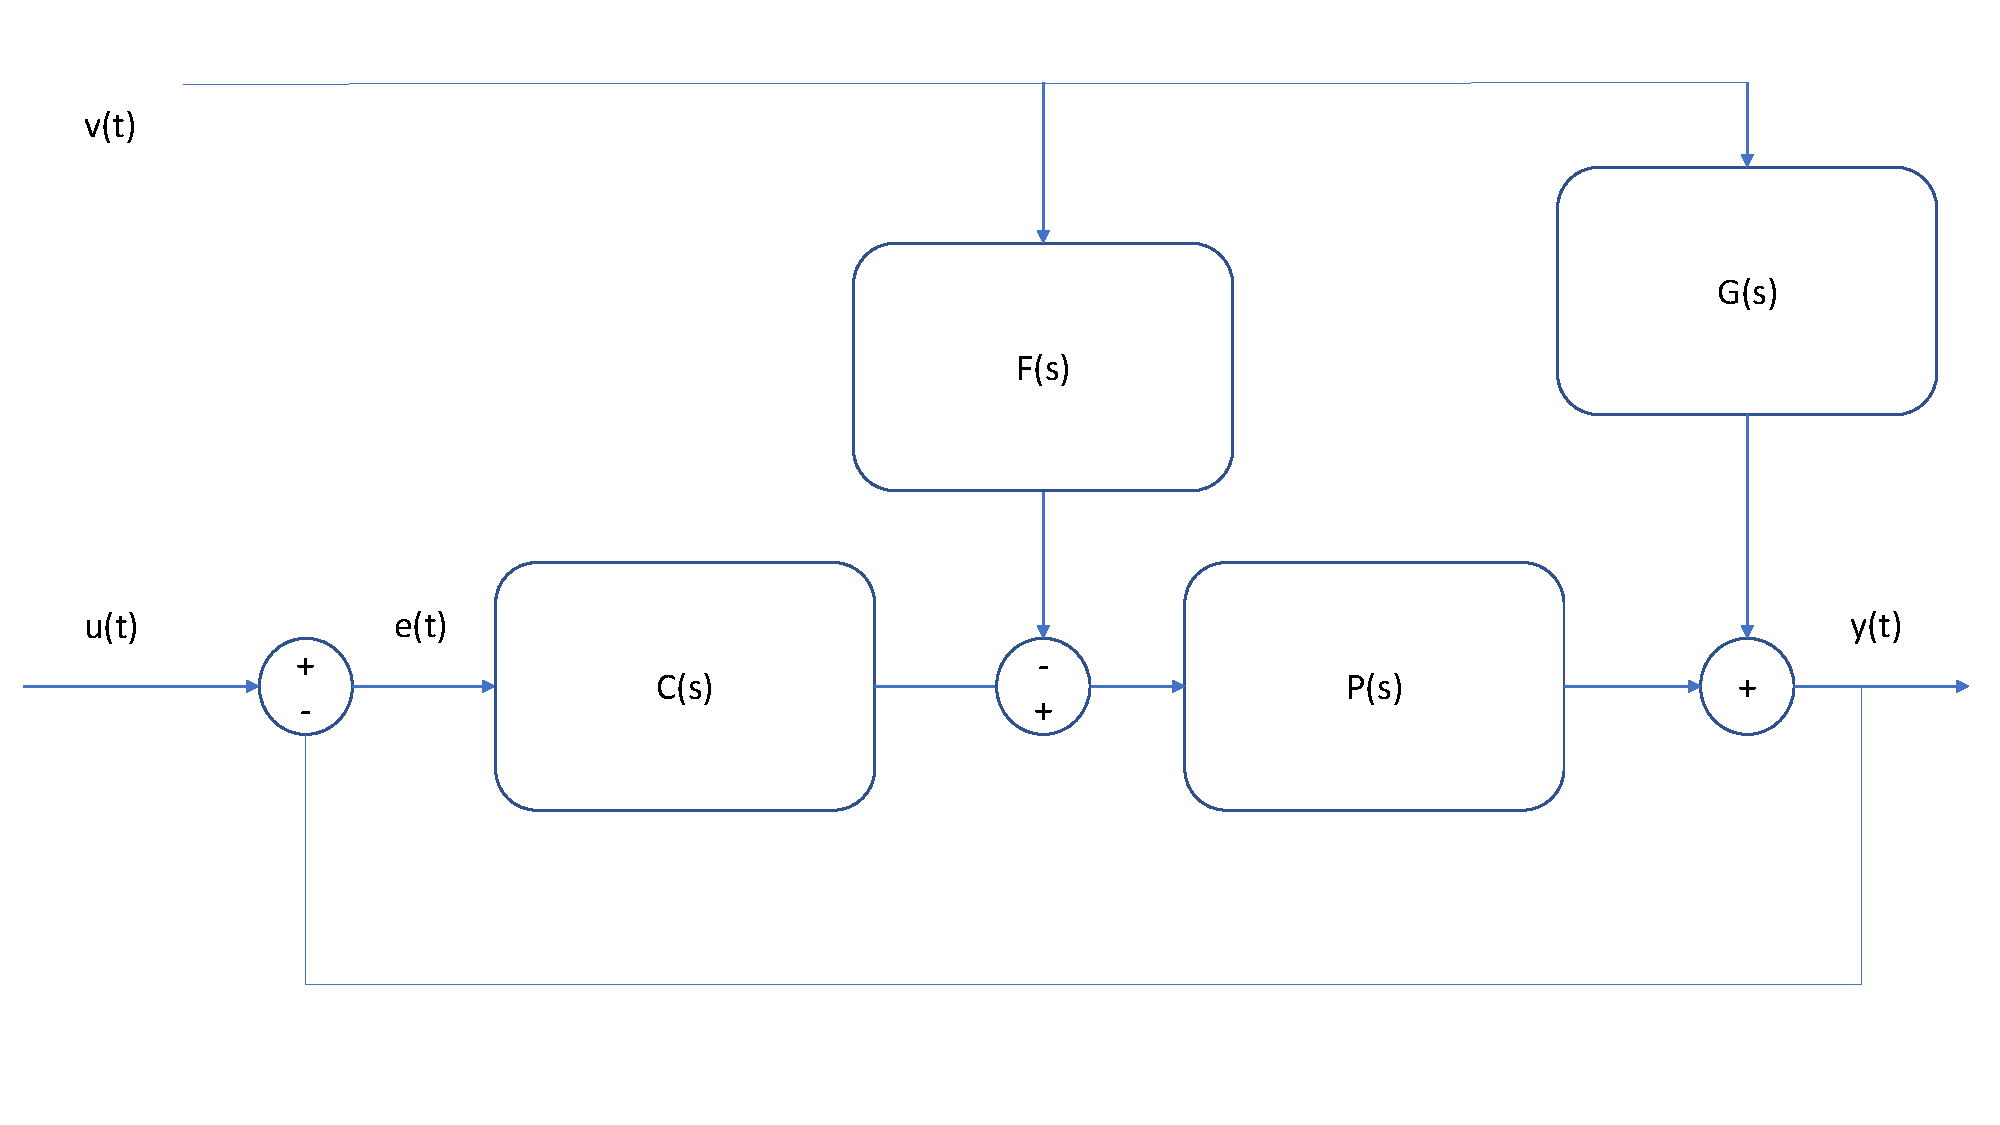
\includegraphics[width=\textwidth]{img/PID-structure.pdf}
    \label{fig:Feed_forward_PID_structure}
    \caption{Comparison of the different controllers with stochastic disturbances}
\end{figure}



